%!TEX encoding = UTF-8 Unicode
\documentclass[onecolumn,12pt]{book}\usepackage[]{graphicx}\usepackage[]{color}
%% maxwidth is the original width if it is less than linewidth
%% otherwise use linewidth (to make sure the graphics do not exceed the margin)
\makeatletter
\def\maxwidth{ %
  \ifdim\Gin@nat@width>\linewidth
    \linewidth
  \else
    \Gin@nat@width
  \fi
}
\makeatother

\definecolor{fgcolor}{rgb}{0.345, 0.345, 0.345}
\newcommand{\hlnum}[1]{\textcolor[rgb]{0.686,0.059,0.569}{#1}}%
\newcommand{\hlstr}[1]{\textcolor[rgb]{0.192,0.494,0.8}{#1}}%
\newcommand{\hlcom}[1]{\textcolor[rgb]{0.678,0.584,0.686}{\textit{#1}}}%
\newcommand{\hlopt}[1]{\textcolor[rgb]{0,0,0}{#1}}%
\newcommand{\hlstd}[1]{\textcolor[rgb]{0.345,0.345,0.345}{#1}}%
\newcommand{\hlkwa}[1]{\textcolor[rgb]{0.161,0.373,0.58}{\textbf{#1}}}%
\newcommand{\hlkwb}[1]{\textcolor[rgb]{0.69,0.353,0.396}{#1}}%
\newcommand{\hlkwc}[1]{\textcolor[rgb]{0.333,0.667,0.333}{#1}}%
\newcommand{\hlkwd}[1]{\textcolor[rgb]{0.737,0.353,0.396}{\textbf{#1}}}%

\usepackage{framed}
\makeatletter
\newenvironment{kframe}{%
 \def\at@end@of@kframe{}%
 \ifinner\ifhmode%
  \def\at@end@of@kframe{\end{minipage}}%
  \begin{minipage}{\columnwidth}%
 \fi\fi%
 \def\FrameCommand##1{\hskip\@totalleftmargin \hskip-\fboxsep
 \colorbox{shadecolor}{##1}\hskip-\fboxsep
     % There is no \\@totalrightmargin, so:
     \hskip-\linewidth \hskip-\@totalleftmargin \hskip\columnwidth}%
 \MakeFramed {\advance\hsize-\width
   \@totalleftmargin\z@ \linewidth\hsize
   \@setminipage}}%
 {\par\unskip\endMakeFramed%
 \at@end@of@kframe}
\makeatother

\definecolor{shadecolor}{rgb}{.97, .97, .97}
\definecolor{messagecolor}{rgb}{0, 0, 0}
\definecolor{warningcolor}{rgb}{1, 0, 1}
\definecolor{errorcolor}{rgb}{1, 0, 0}
\newenvironment{knitrout}{}{} % an empty environment to be redefined in TeX

\usepackage{alltt}
\usepackage[english,italian]{babel}
\usepackage{inconsolata}
%\renewcommand*\familydefault{\ttdefault} %% Only if the base font of the document is to be typewriter style
\usepackage[T1]{fontenc}
\usepackage[buttonsize=1em]{animate}
\usepackage{a4wide,Sweave,url}
\usepackage{verbatim}
\usepackage{makeidx}
\usepackage{babelbib}
\usepackage{float}
\usepackage[T1]{fontenc}
\usepackage[utf8]{inputenc}
\usepackage{framed}
\usepackage{lipsum}
\usepackage[]{color}
\usepackage{graphicx}
\usepackage{fancyvrb}
\usepackage{amsmath}
\usepackage{hyperref}
\newenvironment{question}{\item \textbf{Esercizio}\newline}{}
\newenvironment{solution}{\textbf{Soluzione}\newline}{}
\newenvironment{answerlist}{\renewcommand{\labelenumi}{(\alph{enumi})}\begin{enumerate}}{\end{enumerate}}
\definecolor{grigetto}{rgb}{0.9,0.9,0.9}
 
\DefineVerbatimEnvironment{Sinput}{Verbatim} {xleftmargin=2em} \DefineVerbatimEnvironment{Soutput}{Verbatim}{xleftmargin=2em} \DefineVerbatimEnvironment{Scode}{Verbatim}{xleftmargin=2em} \fvset{listparameters={\setlength{\topsep}{0pt}}} \renewenvironment{Schunk}{\small\vspace{\topsep}}{\vspace{\topsep}\normalsize}
%\usepackage{draftwatermark}
\usepackage{wrapfig}
\usepackage{listings}
\newcounter{fnotes}\setcounter{fnotes}{1}
\newcounter{Raction}\setcounter{Raction}{1}
\newcommand{\varia}[1]{\textsl{\textsf{#1}}}
\newcommand{\mytilde}{$\sim$}
\newcommand{\maurizio}[1]{\color{red}#1 \color{black}}
\newcommand{\federico}[1]{\color{green}#1 \color{black}}
 %\newenvironment{question}{\item \textbf{Problema}\newline}{}
%\newenvironment{solution}{\textbf{Soluzione}\newline}{}
%\DefineVerbatimEnvironment{Sinput}{Verbatim} {xleftmargin=2em,
                                            %  frame=single}
\DefineVerbatimEnvironment{Soutput}{Verbatim}{xleftmargin=2em,   frame=single}
 \newenvironment{ese} [1]{\vskip10pt
%\begin{center}
%\begin{minipage}{12cm}
 \markright{\today}
\colorbox{grigetto}{\parbox{\linewidth}{#1}}}
                          {
                
                          \medskip}
 \newcommand{\virgolette}{\selectlanguage{english}\texttt{"}\selectlanguage{italian}}
 \frontmatter\title{Matematica e Statistica con \textsf{R}}
\author{Federico Comoglio e  Maurizio Rinaldi}
\markright{\today}
\renewcommand{\chaptermark}[1]{%
 \markboth{\chaptername
 \ \thechapter.\ #1}{}}
\newcommand{\rst}{\textsf{RStudio}~}
\newcommand{\rpr}{\textsf{R}~}
\makeindex
\IfFileExists{upquote.sty}{\usepackage{upquote}}{}
\begin{document}
\setkeys{Gin}{width=0.7\textwidth}



\markright{\today}
\thispagestyle{empty}
\maketitle
\newpage
\thispagestyle{empty}
\tableofcontents
\newpage
\thispagestyle{empty}
 \mainmatter

\chapter{Introduzione}
Per accedere ai dati richiesti in questa parte occorre caricare il pacchetto allegato \texttt{libroR}. Per farlo conviene scaricare il file \texttt{libroR$\_0$.0.tgz}  sul proprio computer e  selezionare il menu \texttt{Install}
\begin{center}\begin{figure}[H]
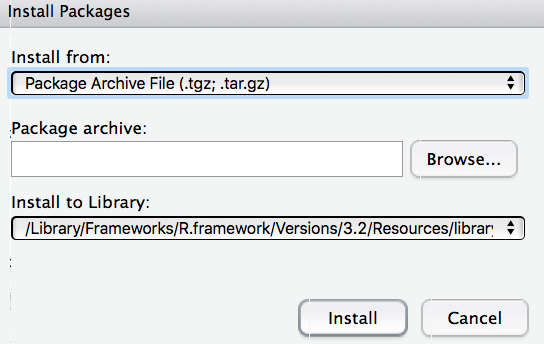
\includegraphics[width=0.4\textwidth]{../grafici/installlibro.png}
\caption{Procedura di installazione del pacchetto}
\label{fig::rlibroinstall} \end{figure}
\end{center}
Il file viene poi localizzato usando \texttt{Browse..}. \\
Alternativamente si pu\`o utilizzare direttamente il comando

\begin{knitrout}
\definecolor{shadecolor}{rgb}{0.969, 0.969, 0.969}\color{fgcolor}\begin{kframe}
\begin{alltt}
\hlkwd{install.packages}\hlstd{(}\hlstr{"libroR_0.0.tgz"}\hlstd{,} \hlkwc{repos} \hlstd{=} \hlkwa{NULL}\hlstd{,} \hlkwc{type} \hlstd{= .Platform}\hlopt{$}\hlstd{pkgType)}
\end{alltt}
\end{kframe}
\end{knitrout}
a patto di impostare la \emph{working directory} precisamente dove si trova il file.
Il pacchetto va poi successivamente caricato con il comando
\begin{knitrout}
\definecolor{shadecolor}{rgb}{0.969, 0.969, 0.969}\color{fgcolor}\begin{kframe}
\begin{alltt}
\hlkwd{library}\hlstd{(}\hlstr{"libroR"}\hlstd{)}
\end{alltt}


{\ttfamily\noindent\itshape\color{messagecolor}{\#\# \\\#\# Attaching package: 'libroR'}}

{\ttfamily\noindent\itshape\color{messagecolor}{\#\# The following objects are masked from 'package:EsamiR':\\\#\# \\\#\#\ \ \ \  meteo, studenti}}\end{kframe}
\end{knitrout}
\begin{figure}
\begin{knitrout}
\definecolor{shadecolor}{rgb}{0.969, 0.969, 0.969}\color{fgcolor}\begin{kframe}
\begin{alltt}
\hlkwd{par}\hlstd{(}\hlkwc{mar} \hlstd{=} \hlkwd{rep}\hlstd{(}\hlnum{3}\hlstd{,} \hlnum{4}\hlstd{))}
\hlkwa{for} \hlstd{(i} \hlkwa{in} \hlkwd{seq}\hlstd{(pi}\hlopt{/}\hlnum{2}\hlstd{,} \hlopt{-}\hlnum{4}\hlopt{/}\hlnum{3} \hlopt{*} \hlstd{pi,} \hlkwc{length} \hlstd{=} \hlnum{12}\hlstd{)) \{}
    \hlkwd{plot}\hlstd{(}\hlnum{0}\hlstd{,} \hlnum{0}\hlstd{,} \hlkwc{pch} \hlstd{=} \hlnum{20}\hlstd{,} \hlkwc{ann} \hlstd{=} \hlnum{FALSE}\hlstd{,} \hlkwc{axes} \hlstd{=} \hlnum{FALSE}\hlstd{)}
    \hlkwd{arrows}\hlstd{(}\hlnum{0}\hlstd{,} \hlnum{0}\hlstd{,} \hlkwd{cos}\hlstd{(i),} \hlkwd{sin}\hlstd{(i))}
    \hlkwd{axis}\hlstd{(}\hlnum{1}\hlstd{,} \hlnum{0}\hlstd{,} \hlstr{"VI"}\hlstd{);} \hlkwd{axis}\hlstd{(}\hlnum{2}\hlstd{,} \hlnum{0}\hlstd{,} \hlstr{"IX"}\hlstd{)}
    \hlkwd{axis}\hlstd{(}\hlnum{3}\hlstd{,} \hlnum{0}\hlstd{,} \hlstr{"XII"}\hlstd{);} \hlkwd{axis}\hlstd{(}\hlnum{4}\hlstd{,} \hlnum{0}\hlstd{,} \hlstr{"III"}\hlstd{);} \hlkwd{box}\hlstd{()}
\hlstd{\}}
\end{alltt}
\end{kframe}











\animategraphics[width=.4\linewidth,controls,loop]{1}{figure/clock-animation-}{1}{12}

\end{knitrout}

\caption{A clock animation. You have to view it in Adobe Reader: click to play/pause;
there are also buttons to speed up or slow down the animation.\label{fig:clock-animation}}
\end{figure}

Precisiamo inoltre che questa \`e una versione assolutamente preliminare.
\chapter{Strutture di dati}

 
Per visualizzare un oggetto di \textsf{R} si pu\`o usare il comando \texttt{print} o il comando \texttt{cat} che fornisce spesso un risultato migliore. \texttt{str} visualizza la struttura di un oggetto mentre \texttt{head} o \texttt{tail} ne visualizzano l'inizio o la fine.


\section{I diversi  tipi di vettori}
\subsection{Vettori di caratteri/stringhe}
Una stringa\index{stringa} di testo \`e una collezione di caratteri; in genere, una stringa \`e resa riconoscibile dall'essere racchiusa tra virgolette.
\subsubsection{Operare con le stringhe}
Oltre alle virgolette, vi sono numerosi altri caratteri speciali che possono apparire in una stringa.
I pi\`u comuni sono ``\texttt{\textbackslash t}'' per \texttt{TAB}, `` \texttt{\textbackslash n}'' per una nuova linea e ``\texttt{\textbackslash }'' per un singolo {\it backslash}.
Quest'ultimo carattere \`e un carattere di \emph{escape} e consente una lettura diversa di quanto lo segue.  Per esempio
\begin{knitrout}
\definecolor{shadecolor}{rgb}{0.969, 0.969, 0.969}\color{fgcolor}\begin{kframe}
\begin{alltt}
\hlkwd{cat}\hlstd{(}\hlstr{"\textbackslash{}"sin\textbackslash{}""}\hlstd{)}
\end{alltt}
\begin{verbatim}
## "sin"
\end{verbatim}
\begin{alltt}
\hlkwd{nchar}\hlstd{(}\hlstr{"\textbackslash{}"sin\textbackslash{}""}\hlstd{)}
\end{alltt}
\begin{verbatim}
## [1] 5
\end{verbatim}
\begin{alltt}
\hlkwd{cat}\hlstd{(}\hlstr{"\textbackslash{}\textbackslash{}"}\hlstd{)}
\end{alltt}
\begin{verbatim}
## \
\end{verbatim}
\begin{alltt}
\hlkwd{cat}\hlstd{(}\hlstr{"ora a capo\textbackslash{}nsono a capo?"}\hlstd{)}
\end{alltt}
\begin{verbatim}
## ora a capo
## sono a capo?
\end{verbatim}
\begin{alltt}
\hlkwd{cat}\hlstd{(}\hlstr{"ora spazio\textbackslash{}triprendo"}\hlstd{)}
\end{alltt}
\begin{verbatim}
## ora spazio	riprendo
\end{verbatim}
\end{kframe}
\end{knitrout}
La funzione \texttt{nchar}, \index{\texttt{nchar}} che conta il numero di caratteri di una stringa, non includer\`a quindi il carattere di \emph{escape}\index{\emph{escape}} nel totale dei caratteri. Ad esempio:
\begin{knitrout}
\definecolor{shadecolor}{rgb}{0.969, 0.969, 0.969}\color{fgcolor}\begin{kframe}
\begin{alltt}
\hlstr{"Tab\textbackslash{}t"}
\end{alltt}
\begin{verbatim}
## [1] "Tab\t"
\end{verbatim}
\begin{alltt}
\hlkwd{cat}\hlstd{(}\hlstr{"Tab\textbackslash{}t"}\hlstd{)}
\end{alltt}
\begin{verbatim}
## Tab	
\end{verbatim}
\begin{alltt}
\hlkwd{nchar}\hlstd{(}\hlstr{"Tab\textbackslash{}t"}\hlstd{)}
\end{alltt}
\begin{verbatim}
## [1] 4
\end{verbatim}
\end{kframe}
\end{knitrout}



Succede spesso di dover lavorare in modo automatico con stringhe di testo, anche nello scrivere indirizzi di rete o cartelle di lavoro. In  \textsf{R} diversi comandi consentono la  generazione, manipolazione e stampa di una o pi\`u stringhe di testo\footnote{Per un  uso pi\`u specifico si pu\`o consultare il pacchetto \texttt{biostrings}.}. Consideriamo inizialmente una singola frase.
%codechunk
\begin{knitrout}
\definecolor{shadecolor}{rgb}{0.969, 0.969, 0.969}\color{fgcolor}\begin{kframe}
\begin{alltt}
\hlstd{x}\hlkwb{=}\hlstr{"lavorare con le stringhe"}
\end{alltt}
\end{kframe}
\end{knitrout}
Possiamo verificarne la classe e determinare il numero di caratteri di \texttt{x}
%codechunk
\begin{knitrout}
\definecolor{shadecolor}{rgb}{0.969, 0.969, 0.969}\color{fgcolor}\begin{kframe}
\begin{alltt}
\hlkwd{class}\hlstd{(x)}
\end{alltt}
\begin{verbatim}
## [1] "character"
\end{verbatim}
\begin{alltt}
\hlkwd{nchar}\hlstd{(x)}
\end{alltt}
\begin{verbatim}
## [1] 24
\end{verbatim}
\end{kframe}
\end{knitrout}
e anche considerare sottostringhe
%codechunk
\begin{knitrout}
\definecolor{shadecolor}{rgb}{0.969, 0.969, 0.969}\color{fgcolor}\begin{kframe}
\begin{alltt}
\hlkwd{substr}\hlstd{(x,}\hlnum{3}\hlstd{,}\hlnum{8}\hlstd{)}
\end{alltt}
\begin{verbatim}
## [1] "vorare"
\end{verbatim}
\end{kframe}
\end{knitrout}
o  abbreviazioni ottenibili con il comando \texttt{abbreviate} \index{\texttt{abbreviate}}
%codechunk
\begin{knitrout}
\definecolor{shadecolor}{rgb}{0.969, 0.969, 0.969}\color{fgcolor}\begin{kframe}
\begin{alltt}
\hlkwd{abbreviate}\hlstd{(}\hlstr{"Mario Rossi"}\hlstd{,}\hlnum{4}\hlstd{)}
\end{alltt}
\begin{verbatim}
## Mario Rossi 
##      "MrRs"
\end{verbatim}
\end{kframe}
\end{knitrout}

Certi oggetti possono essere convertiti a stringhe: per esempio il numero 2 pu\`o essere visto come una stringa e riconvertito a numero.
%codechunk
\begin{knitrout}
\definecolor{shadecolor}{rgb}{0.969, 0.969, 0.969}\color{fgcolor}\begin{kframe}
\begin{alltt}
\hlstd{i}\hlkwb{=}\hlnum{2}\hlstd{;}\hlkwd{toString}\hlstd{(i)}
\end{alltt}
\begin{verbatim}
## [1] "2"
\end{verbatim}
\begin{alltt}
\hlkwd{as.numeric}\hlstd{(}\hlkwd{toString}\hlstd{(i))}
\end{alltt}
\begin{verbatim}
## [1] 2
\end{verbatim}
\end{kframe}
\end{knitrout}
Alcune stringhe molto frequenti sono le lettere \index{\texttt{letters}}\index{\texttt{LETTERS}} dell'alfabeto, maiuscole o minuscole
%codechunk
\begin{knitrout}
\definecolor{shadecolor}{rgb}{0.969, 0.969, 0.969}\color{fgcolor}\begin{kframe}
\begin{alltt}
\hlstd{letters[}\hlnum{1}\hlopt{:}\hlnum{10}\hlstd{]}
\end{alltt}
\begin{verbatim}
##  [1] "a" "b" "c" "d" "e" "f" "g" "h" "i" "j"
\end{verbatim}
\begin{alltt}
\hlstd{LETTERS[}\hlnum{1}\hlopt{:}\hlnum{10}\hlstd{]}
\end{alltt}
\begin{verbatim}
##  [1] "A" "B" "C" "D" "E" "F" "G" "H" "I" "J"
\end{verbatim}
\end{kframe}
\end{knitrout}
o i mesi dell'anno (per esempio abbreviati in inglese)\index{\texttt{month.abb}}
%codechunk

\begin{knitrout}
\definecolor{shadecolor}{rgb}{0.969, 0.969, 0.969}\color{fgcolor}\begin{kframe}
\begin{alltt}
\hlstd{month.abb}
\end{alltt}
\begin{verbatim}
##  [1] "Jan" "Feb" "Mar" "Apr" "May" "Jun" "Jul" "Aug" "Sep"
## [10] "Oct" "Nov" "Dec"
\end{verbatim}
\end{kframe}
\end{knitrout}
Le stringhe possono poi essere ``incollate'' con il comando\index{\texttt{paste}}
%codechunk
\begin{knitrout}
\definecolor{shadecolor}{rgb}{0.969, 0.969, 0.969}\color{fgcolor}\begin{kframe}
\begin{alltt}
\hlkwd{paste}\hlstd{(}\hlstr{"a"}\hlstd{,}\hlstr{"b"}\hlstd{,}\hlkwc{sep}\hlstd{=}\hlstr{""}\hlstd{)}
\end{alltt}
\end{kframe}
\end{knitrout}
dove \texttt{sep}  indica il separatore usato.
E tutto insieme
%codechunk


\begin{knitrout}
\definecolor{shadecolor}{rgb}{0.969, 0.969, 0.969}\color{fgcolor}\begin{kframe}
\begin{alltt}
\hlkwa{for} \hlstd{(i} \hlkwa{in} \hlnum{1}\hlopt{:}\hlnum{5}\hlstd{)} \hlkwd{cat}\hlstd{(}\hlkwd{paste}\hlstd{(}\hlstr{"a"}\hlstd{,}\hlkwd{toString}\hlstd{(i),}\hlstr{"\textbackslash{}t"}\hlstd{,}\hlkwc{sep}\hlstd{=}\hlstr{""}\hlstd{))}
\end{alltt}
\begin{verbatim}
## a1	a2	a3	a4	a5	
\end{verbatim}
\end{kframe}
\end{knitrout}
Il comando pu\`o anche essere utilizzato su vettori.
Per esempio
%codechunk
\begin{knitrout}
\definecolor{shadecolor}{rgb}{0.969, 0.969, 0.969}\color{fgcolor}\begin{kframe}
\begin{alltt}
\hlkwd{paste}\hlstd{(letters[}\hlnum{1}\hlopt{:}\hlnum{10}\hlstd{],}\hlnum{1}\hlopt{:}\hlnum{10}\hlstd{,}\hlkwc{sep}\hlstd{=}\hlstr{""}\hlstd{)}
\end{alltt}
\begin{verbatim}
##  [1] "a1"  "b2"  "c3"  "d4"  "e5"  "f6"  "g7"  "h8"  "i9" 
## [10] "j10"
\end{verbatim}
\end{kframe}
\end{knitrout}
La \textit{recycling rule} continua a valere
%codechunk

\begin{knitrout}
\definecolor{shadecolor}{rgb}{0.969, 0.969, 0.969}\color{fgcolor}\begin{kframe}
\begin{alltt}
\hlkwd{paste}\hlstd{(letters[}\hlnum{1}\hlopt{:}\hlnum{3}\hlstd{],}\hlnum{1}\hlopt{:}\hlnum{10}\hlstd{,}\hlkwc{sep}\hlstd{=}\hlstr{""}\hlstd{)}
\end{alltt}
\begin{verbatim}
##  [1] "a1"  "b2"  "c3"  "a4"  "b5"  "c6"  "a7"  "b8"  "c9" 
## [10] "a10"
\end{verbatim}
\begin{alltt}
\hlkwd{paste}\hlstd{(letters[}\hlnum{1}\hlopt{:}\hlnum{3}\hlstd{],}\hlnum{1}\hlopt{:}\hlnum{12}\hlstd{,}\hlkwc{sep}\hlstd{=}\hlstr{""}\hlstd{)}
\end{alltt}
\begin{verbatim}
##  [1] "a1"  "b2"  "c3"  "a4"  "b5"  "c6"  "a7"  "b8"  "c9" 
## [10] "a10" "b11" "c12"
\end{verbatim}
\end{kframe}
\end{knitrout}
e giocando con \texttt{rep} si possono ottenere diverse combinazioni.
\begin{knitrout}
\definecolor{shadecolor}{rgb}{0.969, 0.969, 0.969}\color{fgcolor}\begin{kframe}
\begin{alltt}
\hlkwd{paste}\hlstd{(}\hlkwd{rep}\hlstd{(letters[}\hlnum{1}\hlopt{:}\hlnum{3}\hlstd{],}\hlkwc{each}\hlstd{=}\hlnum{5}\hlstd{),}\hlnum{1}\hlopt{:}\hlnum{15}\hlstd{,}\hlkwc{sep}\hlstd{=}\hlstr{""}\hlstd{)}
\end{alltt}
\begin{verbatim}
##  [1] "a1"  "a2"  "a3"  "a4"  "a5"  "b6"  "b7"  "b8"  "b9" 
## [10] "b10" "c11" "c12" "c13" "c14" "c15"
\end{verbatim}
\begin{alltt}
\hlkwd{paste}\hlstd{(}\hlkwd{rep}\hlstd{(letters[}\hlnum{1}\hlopt{:}\hlnum{3}\hlstd{],}\hlkwc{ntimes}\hlstd{=}\hlnum{5}\hlstd{),}\hlnum{1}\hlopt{:}\hlnum{15}\hlstd{,}\hlkwc{sep}\hlstd{=}\hlstr{""}\hlstd{)}
\end{alltt}
\begin{verbatim}
##  [1] "a1"  "b2"  "c3"  "a4"  "b5"  "c6"  "a7"  "b8"  "c9" 
## [10] "a10" "b11" "c12" "a13" "b14" "c15"
\end{verbatim}
\end{kframe}
\end{knitrout}
Con l'opzione \texttt{collapse="x"} le stringhe vengono unite con separatore la stringa "x".
%codechunk
\begin{knitrout}
\definecolor{shadecolor}{rgb}{0.969, 0.969, 0.969}\color{fgcolor}\begin{kframe}
\begin{alltt}
\hlkwd{paste}\hlstd{(}\hlkwd{c}\hlstd{(}\hlstr{"X"}\hlstd{,} \hlstr{"Y"}\hlstd{),} \hlnum{1}\hlopt{:}\hlnum{4}\hlstd{,} \hlkwc{sep} \hlstd{=} \hlstr{"-"}\hlstd{,} \hlkwc{collapse} \hlstd{=} \hlstr{"--"}\hlstd{)}
\end{alltt}
\begin{verbatim}
## [1] "X-1--Y-2--X-3--Y-4"
\end{verbatim}
\end{kframe}
\end{knitrout}
Si noti il separatore - dell'operazione \texttt{paste} e  - - dell'operazione \texttt{collapse}.

 \begin{shaded}
 \begin{enumerate}
 \item{} Inserisci il tuo cognome in una variabile `cognome' ed il tuo nome in una variabile 'nome'. Crea una terza variabile 'nomecognome' che contenga entrambi separati da un TAB. Stampa a console la scritta "Good job" seguita dal valore di nomecognome.
  \item{} Creare un elenco che contenga mesi e anno dal 2001 al 2010 nel seguente formato "tre lettere iniziali del mese-anno".
 \item{} Costruire una tabella che contenga tutte le parole di 2 lettere.
\item{}
Si consideri
\begin{knitrout}
\definecolor{shadecolor}{rgb}{0.969, 0.969, 0.969}\color{fgcolor}\begin{kframe}
\begin{alltt}
\hlkwd{paste}\hlstd{(letters[}\hlnum{1}\hlopt{:}\hlnum{7}\hlstd{],}\hlnum{1}\hlopt{:}\hlnum{7}\hlstd{,}\hlkwc{sep}\hlstd{=}\hlstr{"="}\hlstd{)}
\end{alltt}
\end{kframe}
\end{knitrout}
Estendere la corrispondenza a tutto l'alfabeto.
\item Creare un elenco in cui a ciascun mese corrisponda il suo numero (a partire da gennaio).
\item Creare un elenco con nomi i mesi e valori il numero di giorni di ciascun mese.
\item Scrivere un elenco di 5 persone con le relative date di nascita nel formato anno-mese-giorno.
 \end{enumerate}
 \end{shaded}
\subsection{Vettori logici}
I valori logici in R sono i valori \texttt{TRUE} e \texttt{FALSE} e corrispondono alla veridicit\`a di un'affermazione.
Per esempio
\begin{knitrout}
\definecolor{shadecolor}{rgb}{0.969, 0.969, 0.969}\color{fgcolor}\begin{kframe}
\begin{alltt}
\hlnum{1}\hlopt{:}\hlnum{10} \hlopt{>} \hlnum{4}
\end{alltt}
\begin{verbatim}
##  [1] FALSE FALSE FALSE FALSE  TRUE  TRUE  TRUE  TRUE  TRUE
## [10]  TRUE
\end{verbatim}
\end{kframe}
\end{knitrout}
Ci fornisce simultaneamente i valori dei 10 confronti.
\section{Vettori numerici e operazioni di aritmetica modulare}
\begin{knitrout}
\definecolor{shadecolor}{rgb}{0.969, 0.969, 0.969}\color{fgcolor}\begin{kframe}
\begin{alltt}
\hlnum{1}\hlopt{:}\hlnum{10}
\end{alltt}
\begin{verbatim}
##  [1]  1  2  3  4  5  6  7  8  9 10
\end{verbatim}
\end{kframe}
\end{knitrout}
\begin{knitrout}
\definecolor{shadecolor}{rgb}{0.969, 0.969, 0.969}\color{fgcolor}\begin{kframe}
\begin{alltt}
\hlstd{resto}\hlkwb{=}\hlstd{(}\hlnum{1}\hlopt{:}\hlnum{10}\hlstd{)}\hlopt\hlnum{4}
\hlstd{resto}
\end{alltt}
\begin{verbatim}
##  [1] 1 2 3 0 1 2 3 0 1 2
\end{verbatim}
\begin{alltt}
\hlstd{quoziente}\hlkwb{=}\hlstd{(}\hlnum{1}\hlopt{:}\hlnum{10}\hlstd{)}\hlopt\hlnum{4}
\hlstd{quoziente}
\end{alltt}
\begin{verbatim}
##  [1] 0 0 0 1 1 1 1 2 2 2
\end{verbatim}
\begin{alltt}
\hlstd{resto}\hlopt{+}\hlnum{4}\hlopt{*}\hlstd{quoziente}
\end{alltt}
\begin{verbatim}
##  [1]  1  2  3  4  5  6  7  8  9 10
\end{verbatim}
\end{kframe}
\end{knitrout}
\section{Matrici}

Assegnati $n\times m$ ingressi possiamo costruire una matrice (ossia una tabella) con $n$ righe e $m$ colonne. Occorre solo riempire la matrice per righe o per colonne.
Ad esempio:
%code chunk
\begin{knitrout}
\definecolor{shadecolor}{rgb}{0.969, 0.969, 0.969}\color{fgcolor}\begin{kframe}
\begin{alltt}
\hlstd{a}\hlkwb{<-}\hlkwd{matrix}\hlstd{(letters[}\hlnum{1}\hlopt{:}\hlnum{12}\hlstd{],}\hlkwc{nrow}\hlstd{=}\hlnum{3}\hlstd{,}\hlkwc{ncol}\hlstd{=}\hlnum{4}\hlstd{)}
\hlstd{a}
\end{alltt}
\begin{verbatim}
##      [,1] [,2] [,3] [,4]
## [1,] "a"  "d"  "g"  "j" 
## [2,] "b"  "e"  "h"  "k" 
## [3,] "c"  "f"  "i"  "l"
\end{verbatim}
\begin{alltt}
\hlkwd{class}\hlstd{(a)}
\end{alltt}
\begin{verbatim}
## [1] "matrix"
\end{verbatim}
\end{kframe}
\end{knitrout}
Se i parametri hanno natura diversa vengono resi uniformi
%code chunk
\begin{knitrout}
\definecolor{shadecolor}{rgb}{0.969, 0.969, 0.969}\color{fgcolor}\begin{kframe}
\begin{alltt}
\hlstd{a}\hlkwb{<-}\hlkwd{matrix}\hlstd{(}\hlkwd{c}\hlstd{(}\hlnum{1}\hlopt{:}\hlnum{6}\hlstd{,letters[}\hlnum{1}\hlopt{:}\hlnum{6}\hlstd{]),}\hlkwc{nrow}\hlstd{=}\hlnum{3}\hlstd{,}\hlkwc{ncol}\hlstd{=}\hlnum{4}\hlstd{);a}
\end{alltt}
\begin{verbatim}
##      [,1] [,2] [,3] [,4]
## [1,] "1"  "4"  "a"  "d" 
## [2,] "2"  "5"  "b"  "e" 
## [3,] "3"  "6"  "c"  "f"
\end{verbatim}
\end{kframe}
\end{knitrout}
Con il parametro \texttt{byrow=T} il riempimento avviene per righe, anzich\`e per colonne.
%code chunk
\begin{knitrout}
\definecolor{shadecolor}{rgb}{0.969, 0.969, 0.969}\color{fgcolor}\begin{kframe}
\begin{alltt}
 \hlstd{a}\hlkwb{<-}\hlkwd{matrix}\hlstd{(}\hlnum{1}\hlopt{:}\hlnum{12}\hlstd{,}\hlkwc{nrow}\hlstd{=}\hlnum{3}\hlstd{,}\hlkwc{ncol}\hlstd{=}\hlnum{4}\hlstd{,}\hlkwc{byrow}\hlstd{=T)}
 \hlstd{a}
\end{alltt}
\begin{verbatim}
##      [,1] [,2] [,3] [,4]
## [1,]    1    2    3    4
## [2,]    5    6    7    8
## [3,]    9   10   11   12
\end{verbatim}
\end{kframe}
\end{knitrout}
Se i numeri sono insufficienti vengono \emph {riciclati}
%code chunk
\begin{knitrout}
\definecolor{shadecolor}{rgb}{0.969, 0.969, 0.969}\color{fgcolor}\begin{kframe}
\begin{alltt}
\hlstd{a}\hlkwb{<-}\hlkwd{matrix}\hlstd{(}\hlnum{1}\hlopt{:}\hlnum{4}\hlstd{,}\hlkwc{nrow}\hlstd{=}\hlnum{3}\hlstd{,}\hlkwc{ncol}\hlstd{=}\hlnum{4}\hlstd{)}
\hlstd{a}
\end{alltt}
\begin{verbatim}
##      [,1] [,2] [,3] [,4]
## [1,]    1    4    3    2
## [2,]    2    1    4    3
## [3,]    3    2    1    4
\end{verbatim}
\end{kframe}
\end{knitrout}
in modo pacifico se sono un sottomultiplo della dimensione della matrice o con qualche
\texttt{warning} altrimenti.
%code chunk
\begin{knitrout}
\definecolor{shadecolor}{rgb}{0.969, 0.969, 0.969}\color{fgcolor}\begin{kframe}
\begin{alltt}
\hlstd{a}\hlkwb{<-}\hlkwd{matrix}\hlstd{(}\hlnum{2}\hlstd{,}\hlkwc{nrow}\hlstd{=}\hlnum{3}\hlstd{,}\hlkwc{ncol}\hlstd{=}\hlnum{4}\hlstd{)}
\hlstd{a}
\end{alltt}
\end{kframe}
\end{knitrout}
Si possono anche definire gli ingressi attraverso opportune funzioni
%code chunk

\begin{knitrout}
\definecolor{shadecolor}{rgb}{0.969, 0.969, 0.969}\color{fgcolor}\begin{kframe}
\begin{alltt}
\hlkwa{for}\hlstd{(j} \hlkwa{in} \hlstd{(}\hlnum{1}\hlopt{:}\hlnum{4}\hlstd{))} \hlkwa{for}\hlstd{(i} \hlkwa{in} \hlstd{(}\hlnum{1}\hlopt{:}\hlnum{3}\hlstd{))  a[i,j]}\hlkwb{<-}\hlstd{i}\hlopt{^}\hlnum{2}\hlopt{+}\hlstd{j}
\end{alltt}
\end{kframe}
\end{knitrout}
Per assegnare nomi alle  righe e alle colonne:\index{\texttt{colnames}} \index{\texttt{rownames}}
\begin{eqnarray*}
 \texttt{colnames}(\varia{matrice})=\texttt{c}(\virgolette \varia{  nome}_1\virgolette,\\
\virgolette \varia{nome}_2\virgolette,\ldots,\virgolette \varia{nome}_n\virgolette )\\
 \texttt{rownames}(\varia{matrice})=\texttt{c}(\virgolette \varia{nome}_1\virgolette,\\
\virgolette \varia{nome}_2\virgolette,\ldots,\virgolette \varia{nome}_n\virgolette )
\end{eqnarray*}
\begin{knitrout}
\definecolor{shadecolor}{rgb}{0.969, 0.969, 0.969}\color{fgcolor}\begin{kframe}
\begin{alltt}
\hlkwd{colnames}\hlstd{(a)}\hlkwb{=}\hlkwd{c}\hlstd{(}\hlstr{"c1"}\hlstd{,}\hlstr{"c2"}\hlstd{,}\hlstr{"c3"}\hlstd{,}\hlstr{"c4"}\hlstd{)}
\hlkwd{rownames}\hlstd{(a)}\hlkwb{=}\hlkwd{c}\hlstd{(}\hlstr{"r1"}\hlstd{,}\hlstr{"r2"}\hlstd{,}\hlstr{"r3"}\hlstd{)}
\hlstd{a}
\end{alltt}
\begin{verbatim}
##    c1 c2 c3 c4
## r1  1  4  3  2
## r2  2  1  4  3
## r3  3  2  1  4
\end{verbatim}
\end{kframe}
\end{knitrout}
\subsubsection{Aggiungere righe o colonne}
Per aggiungere una o pi\`u righe (o colonne)
ad una matrice si possono usare i comandi (\texttt{rbind} e \texttt{cbind})
\begin{knitrout}
\definecolor{shadecolor}{rgb}{0.969, 0.969, 0.969}\color{fgcolor}\begin{kframe}
\begin{alltt}
\hlkwd{dim}\hlstd{(a)}
\end{alltt}
\begin{verbatim}
## [1] 3 4
\end{verbatim}
\begin{alltt}
\hlkwd{rbind}\hlstd{(a,letters[}\hlnum{1}\hlopt{:}\hlkwd{ncol}\hlstd{(a)])}
\end{alltt}
\begin{verbatim}
##    c1  c2  c3  c4 
## r1 "1" "4" "3" "2"
## r2 "2" "1" "4" "3"
## r3 "3" "2" "1" "4"
##    "a" "b" "c" "d"
\end{verbatim}
\begin{alltt}
\hlkwd{cbind}\hlstd{(a,letters[}\hlnum{1}\hlopt{:}\hlkwd{nrow}\hlstd{(a)])}
\end{alltt}
\begin{verbatim}
##    c1  c2  c3  c4     
## r1 "1" "4" "3" "2" "a"
## r2 "2" "1" "4" "3" "b"
## r3 "3" "2" "1" "4" "c"
\end{verbatim}
\end{kframe}
\end{knitrout}
Possiamo anche effettuare semplici operazioni, come somma degli elementi delle righe o delle colonne
\begin{knitrout}
\definecolor{shadecolor}{rgb}{0.969, 0.969, 0.969}\color{fgcolor}\begin{kframe}
\begin{alltt}
\hlkwd{colSums}\hlstd{(a)}
\end{alltt}
\begin{verbatim}
## c1 c2 c3 c4 
##  6  7  8  9
\end{verbatim}
\begin{alltt}
\hlkwd{rowSums}\hlstd{(a)}
\end{alltt}
\begin{verbatim}
## r1 r2 r3 
## 10 10 10
\end{verbatim}
\end{kframe}
\end{knitrout}

\subsection{Operazioni con le matrici}
\subsubsection{Trasposizione}
Per invertire righe e colonne di una matrice ossia per ottenere il trasposto \index{trasposto} di una matrice si usa il comando \texttt{t}(\texttt{matrice})\index{\texttt{t}, trasposto}
%code chunk
\begin{knitrout}
\definecolor{shadecolor}{rgb}{0.969, 0.969, 0.969}\color{fgcolor}\begin{kframe}
\begin{alltt}
\hlkwd{t}\hlstd{(a)}
\end{alltt}
\begin{verbatim}
##    r1 r2 r3
## c1  1  2  3
## c2  4  1  2
## c3  3  4  1
## c4  2  3  4
\end{verbatim}
\end{kframe}
\end{knitrout}
\subsubsection{Prodotto}
Per la  moltiplicazione di matrici (definita per ingressi numerici) si usa il simbolo \texttt{\%*\%}.
\index{\texttt{\%*\%}, prodotto di matrici}
 %code chunk
\begin{knitrout}
\definecolor{shadecolor}{rgb}{0.969, 0.969, 0.969}\color{fgcolor}\begin{kframe}
\begin{alltt}
\hlstd{b}\hlkwb{<-}\hlkwd{matrix}\hlstd{(}\hlnum{2}\hlstd{,}\hlkwc{nrow}\hlstd{=}\hlnum{3}\hlstd{,}\hlkwc{ncol}\hlstd{=}\hlnum{3}\hlstd{)}
\hlkwa{for}\hlstd{(j} \hlkwa{in} \hlstd{(}\hlnum{1}\hlopt{:}\hlnum{3}\hlstd{))}
\hlkwa{for}\hlstd{(i} \hlkwa{in} \hlstd{(}\hlnum{1}\hlopt{:}\hlnum{3}\hlstd{)) b[i,j]}\hlkwb{<-}\hlstd{i}\hlopt{+}\hlstd{j}\hlopt{+}\hlstd{i}\hlopt{^}\hlnum{2}
\hlstd{b}
\end{alltt}
\begin{verbatim}
##      [,1] [,2] [,3]
## [1,]    3    4    5
## [2,]    7    8    9
## [3,]   13   14   15
\end{verbatim}
\end{kframe}
\end{knitrout}
Non \`e infatti possibile moltiplicare una matrice 3x4 con una 3x3. Possiamo per\`o calcolare
%code chunk
\begin{knitrout}
\definecolor{shadecolor}{rgb}{0.969, 0.969, 0.969}\color{fgcolor}\begin{kframe}
\begin{alltt}
\hlstd{b}\hlopt\hlstd{a}
\end{alltt}
\begin{verbatim}
##      c1 c2  c3  c4
## [1,] 26 26  30  38
## [2,] 50 54  62  74
## [3,] 86 96 110 128
\end{verbatim}
\end{kframe}
\end{knitrout}
\subsubsection{Determinante} Il determinante di una matrice quadrata si ottiene con il comando
%\index{\texttt{det},determinante}
\begin{equation}\texttt{det} (\varia{matrice})\end{equation}
\begin{knitrout}
\definecolor{shadecolor}{rgb}{0.969, 0.969, 0.969}\color{fgcolor}\begin{kframe}
\begin{alltt}
\hlkwd{det}\hlstd{(b)}
\end{alltt}
\begin{verbatim}
## [1] 1.887379e-14
\end{verbatim}
\end{kframe}
\end{knitrout}

Si noti che se eseguendo i calcoli a mano si trovano in alcuni casi risultati diversi da quelli di {\textsf R}. Per esempio la matrice in esame ha determinante 0 e 0 ne \`e anche un autovalore.\index{autovalore}
\begin{shaded}
 \begin{enumerate}
 \item{}Creare una matrice $3\times 2$ che abbia come ingressi i primi 6 numeri pari. Estendere la matrice aggiungendo due colonne contenenti i primi 6 numeri dispari. Calcolare e stampare la somma per riga e la somma per colonna. Modifica la matrice cambiando di segno la prima riga. Moltiplicare la matrice  per 4.
 \end{enumerate}
 \end{shaded}
 \section{I \emph{dataframe}}

I \emph{dataframe} (in \rpr  \texttt{data.frame}) costituiscono in \rpr la classe di oggetti fondamentali per la collezione di dati per una susseguente analisi statistica.
Un \emph{dataframe}  \`e una collezione di vettori aventi egual lunghezza e allineati verticalmente. Un dataframe \`e diverso da una matrice in quanto le colonne sono vettori eventualmente di tipi diversi. Il comando generale per costruire \emph{dataframe} a partire da vettori o liste
\`e \texttt{data.frame}.  Esso richiede come parametri i nomi dei vettori (colonna) da affiancare nella tabella. In generale si scrive:
\begin{equation*}\texttt{data.frame}(\varia{vettore}_1,\varia{vettore}_2, \ldots, \varia{vettore}_n)\end{equation*}
dove tutti i vettori hanno la stessa lunghezza.
Si noti la asimmetria  (rispetto ad una matrice) nel ruolo di righe e colonne. Le colonne sono omogenee, lo stesso non si pu\`o dire per le righe. Le colonne sono le variabili analizzate, le righe le unit\`a statistiche. Anche i vari comandi che vedremo rispettano tale differenza.
Il data.frame classico da cui partiamo è \texttt{iris}

Per avere una stampa abbreviata
%codechunk

\begin{knitrout}
\definecolor{shadecolor}{rgb}{0.969, 0.969, 0.969}\color{fgcolor}\begin{kframe}
\begin{alltt}
\hlkwd{head}\hlstd{(iris)}
\end{alltt}
\begin{verbatim}
##   Sepal.Length Sepal.Width Petal.Length Petal.Width Species
## 1          5.1         3.5          1.4         0.2  setosa
## 2          4.9         3.0          1.4         0.2  setosa
## 3          4.7         3.2          1.3         0.2  setosa
## 4          4.6         3.1          1.5         0.2  setosa
## 5          5.0         3.6          1.4         0.2  setosa
## 6          5.4         3.9          1.7         0.4  setosa
\end{verbatim}
\begin{alltt}
\hlkwd{tail}\hlstd{(iris)}
\end{alltt}
\begin{verbatim}
##     Sepal.Length Sepal.Width Petal.Length Petal.Width
## 145          6.7         3.3          5.7         2.5
## 146          6.7         3.0          5.2         2.3
## 147          6.3         2.5          5.0         1.9
## 148          6.5         3.0          5.2         2.0
## 149          6.2         3.4          5.4         2.3
## 150          5.9         3.0          5.1         1.8
##       Species
## 145 virginica
## 146 virginica
## 147 virginica
## 148 virginica
## 149 virginica
## 150 virginica
\end{verbatim}
\end{kframe}
\end{knitrout}

Il comando \texttt{str}\index{\texttt{str}} consente una visualizzazione parziale che ci fornisce la struttura.
 
\small
\begin{knitrout}
\definecolor{shadecolor}{rgb}{0.969, 0.969, 0.969}\color{fgcolor}\begin{kframe}
\begin{verbatim}
## 'data.frame':	150 obs. of  5 variables:
##  $ Sepal.Length: num  5.1 4.9 4.7 4.6 5 5.4 4.6 5 4.4 4.9 ...
##  $ Sepal.Width : num  3.5 3 3.2 3.1 3.6 3.9 3.4 3.4 2.9 3.1 ...
##  $ Petal.Length: num  1.4 1.4 1.3 1.5 1.4 1.7 1.4 1.5 1.4 1.5 ...
##  $ Petal.Width : num  0.2 0.2 0.2 0.2 0.2 0.4 0.3 0.2 0.2 0.1 ...
##  $ Species     : Factor w/ 3 levels "setosa","versicolor",..: 1 1 1 1 1 1 1 1 1 1 ...
\end{verbatim}
\end{kframe}
\end{knitrout}
\normalsize
Per esempio possiamo considerare il dataframe \texttt{d} definito come segue 
\begin{knitrout}
\definecolor{shadecolor}{rgb}{0.969, 0.969, 0.969}\color{fgcolor}\begin{kframe}
\begin{alltt}
\hlstd{L3} \hlkwb{<-} \hlstd{LETTERS[}\hlnum{1}\hlopt{:}\hlnum{3}\hlstd{]}
\hlstd{d} \hlkwb{<-} \hlkwd{data.frame}\hlstd{(}\hlkwd{cbind}\hlstd{(}\hlkwc{x}\hlstd{=}\hlnum{1}\hlstd{,} \hlkwc{y}\hlstd{=}\hlnum{1}\hlopt{:}\hlnum{10}\hlstd{,}
\hlkwc{fac}\hlstd{=}\hlkwd{sample}\hlstd{(L3,} \hlnum{10}\hlstd{,} \hlkwc{replace}\hlstd{=}\hlnum{TRUE}\hlstd{)),}
\hlkwc{stringsAsFactors}\hlstd{=}\hlnum{TRUE}\hlstd{)}
\hlstd{d}
\end{alltt}
\begin{verbatim}
##    x  y fac
## 1  1  1   A
## 2  1  2   C
## 3  1  3   A
## 4  1  4   C
## 5  1  5   C
## 6  1  6   B
## 7  1  7   C
## 8  1  8   B
## 9  1  9   A
## 10 1 10   B
\end{verbatim}
\end{kframe}
\end{knitrout}
Si noti che anche in questo caso si usa la \emph{recycling rule}

In quanto segue lavoreremo con il seguente \emph{dataframe} che rappresenta i risultati di un'indagine svolta sugli studenti che nell'Anno Accademico 2007/2008 frequentavano il primo anno del corso di Laurea di Farmacia della Facolt\`a di Farmacia del Piemonte Orientale. Potete caricarlo  in {\textsf R} dal pacchetto con il comando
%code chunk

\begin{knitrout}
\definecolor{shadecolor}{rgb}{0.969, 0.969, 0.969}\color{fgcolor}\begin{kframe}
\begin{alltt}
\hlkwd{data}\hlstd{(farmacia)}
\end{alltt}
\end{kframe}
\end{knitrout}
Il comando \texttt{colnames}  consente di  visualizzare o assegnare il nome alle colonne.
Per esempio
%code chunk
\begin{knitrout}
\definecolor{shadecolor}{rgb}{0.969, 0.969, 0.969}\color{fgcolor}\begin{kframe}
\begin{alltt}
\hlkwd{colnames}\hlstd{(farmacia)}
\end{alltt}
\begin{verbatim}
## [1] "Sex"  "W"    "H"    "Eyes" "Hair" "Sh"   "hM"  
## [8] "hF"
\end{verbatim}
\end{kframe}
\end{knitrout}
Le varie colonne hanno dei nomi di facile interpretazione. Si noti anche che a fianco di variabili numeriche (\texttt{W} e \texttt{H}, peso-altezza ad esempio) sono presenti variabili  \emph {nominali} quali sesso (\texttt{Sex}) e colore degli occhi (\texttt{Eyes}).
Per associare i nomi alle colonne  alle varie colonne dobbiamo eseguire una operazione di collegamento con il comando \texttt{attach},
%code chunk
\begin{knitrout}
\definecolor{shadecolor}{rgb}{0.969, 0.969, 0.969}\color{fgcolor}\begin{kframe}
\begin{alltt}
\hlkwd{attach}\hlstd{(farmacia)}
\end{alltt}
\end{kframe}
\end{knitrout}
A questo punto digitando il nome delle colonne appare il contenuto della colonna
%code chunk
\begin{knitrout}
\definecolor{shadecolor}{rgb}{0.969, 0.969, 0.969}\color{fgcolor}\begin{kframe}
\begin{alltt}
\hlstd{Sex}
\end{alltt}
\begin{verbatim}
##  [1] F M M M F M F F M F F F F F M F F F M M M F F F F
## [26] F M F M M F F M M F F F F M F M M F F F F F F F M
## [51] M M F F M
## Levels: F M
\end{verbatim}
\end{kframe}
\end{knitrout}
Le variabili nominali sono caratterizzate dal fatto che i loro valori (livelli, \texttt{levels}) \index{\texttt{level}} non hanno significato numerico, anche se possono essere codificati con dei numeri.   Ad esempio il sesso di una persona \`e una variabile nominale con due possibili valori, che sono stati  indicati qui con la convenzione  \texttt{"F"}  per le femmine e \texttt{"M"} per i maschi.  Se volessimo eliminare i livelli di una variabile nominale potremmo scrivere
\begin{knitrout}
\definecolor{shadecolor}{rgb}{0.969, 0.969, 0.969}\color{fgcolor}\begin{kframe}
\begin{alltt}
\hlstd{Sex}\hlkwb{=}\hlkwd{as.vector}\hlstd{(Sex)}
\hlstd{Sex}
\end{alltt}
\begin{verbatim}
##  [1] "F" "M" "M" "M" "F" "M" "F" "F" "M" "F" "F" "F"
## [13] "F" "F" "M" "F" "F" "F" "M" "M" "M" "F" "F" "F"
## [25] "F" "F" "M" "F" "M" "M" "F" "F" "M" "M" "F" "F"
## [37] "F" "F" "M" "F" "M" "M" "F" "F" "F" "F" "F" "F"
## [49] "F" "M" "M" "M" "F" "F" "M"
\end{verbatim}
\begin{alltt}
\hlkwd{class}\hlstd{(Sex)}
\end{alltt}
\begin{verbatim}
## [1] "character"
\end{verbatim}
\end{kframe}
\end{knitrout}
Possiamo anche considerare il processo inverso e cambiare una variabile priva di livelli in una nominale
$$\texttt{factor}(\varia{variabile})\rightarrow\varia{ variabile}$$
Per definire i suoi livelli (ad esempio $n$) scriveremo:
$$\texttt{levels}(\varia{variabile})\leftarrow\texttt{c}(\varia{nome}_1,\varia{nome}_2,\ldots,\varia{nome}_n)$$
Per rendere la variabilie \texttt{Sex} nominale con nomi dei livelli
\texttt{F} e \texttt{M})  scriveremo:
\begin{knitrout}
\definecolor{shadecolor}{rgb}{0.969, 0.969, 0.969}\color{fgcolor}\begin{kframe}
\begin{alltt}
\hlstd{Sex}\hlkwb{=}\hlkwd{factor}\hlstd{(Sex)}
\hlstd{Sex}
\end{alltt}
\begin{verbatim}
##  [1] F M M M F M F F M F F F F F M F F F M M M F F F F
## [26] F M F M M F F M M F F F F M F M M F F F F F F F M
## [51] M M F F M
## Levels: F M
\end{verbatim}
\end{kframe}
\end{knitrout}
Con il comando
\texttt{detach} \index{detach}  si pu\`o eliminare l'associazione creata tra colonne e nomi delle colonne.
Consideriamo ora un \emph{dataset} simile raccolto dagli studenti di Biotecnologie dello stesso anno
%code chunk


Scrivendo
\begin{knitrout}
\definecolor{shadecolor}{rgb}{0.969, 0.969, 0.969}\color{fgcolor}\begin{kframe}
\begin{alltt}
\hlkwd{class}\hlstd{(biotec)}
\end{alltt}
\begin{verbatim}
## [1] "data.frame"
\end{verbatim}
\end{kframe}
\end{knitrout}
vediamo che anche \texttt{biotec} \`e un \emph{dataframe}.  Inoltre confrontando i nomi delle colonne di \texttt{farmacia} e di \texttt{biotec} possiamo verificare che sono essenzialmente uguali a meno di traduzione e eventuale abbreviazione.
Possiamo creare un \emph{dataframe} unico che raggruppi \texttt{biotec} e \texttt{farmacia}. Per farlo  vorremmo incollare un \emph{dataframe} sopra all'altro.
A tal fine occorre uniformare i nomi delle colonne scrivendo per esempio
\begin{knitrout}
\definecolor{shadecolor}{rgb}{0.969, 0.969, 0.969}\color{fgcolor}\begin{kframe}
\begin{alltt}
\hlkwd{colnames}\hlstd{(biotec)}\hlkwb{=}\hlkwd{colnames}\hlstd{(farmacia)}
\hlstd{studenti}\hlkwb{=}\hlkwd{rbind}\hlstd{(farmacia,biotec)}
\hlkwd{head}\hlstd{(studenti)}
\end{alltt}
\begin{verbatim}
##   Sex  W    H     Eyes    Hair Sh   hM   hF
## 1   F 62 1.75  CASTANI CASTANI 40 1.77 1.78
## 2   M 64 1.84  CASTANI CASTANI 43 1.72 1.80
## 3   M 80 1.70  CASTANI CASTANI 44 1.65 1.73
## 4   M 80 1.75  CASTANI    NERI 44 1.66 1.78
## 5   F 50 1.70 NOCCIOLA    NERI 38 1.65 1.79
## 6   M 63 1.88  CASTANI  BIONDI 44 1.58 1.75
\end{verbatim}
\end{kframe}
\end{knitrout}
Si noti che il comando \texttt{rbind} \index{\texttt{rbind}} incolla per riga, mentre l'analogo comando \texttt{cbind}
\index{\texttt{cbind}} incolla le colonne.
Le intestazioni di riga di dati sono
\begin{knitrout}
\definecolor{shadecolor}{rgb}{0.969, 0.969, 0.969}\color{fgcolor}\begin{kframe}
\begin{alltt}
\hlkwd{rownames}\hlstd{(studenti)}
\end{alltt}
\begin{verbatim}
##  [1] "1"   "2"   "3"   "4"   "5"   "6"   "7"  
##  [8] "8"   "9"   "10"  "11"  "12"  "13"  "14" 
## [15] "15"  "16"  "17"  "18"  "19"  "20"  "21" 
## [22] "22"  "23"  "24"  "25"  "26"  "27"  "28" 
## [29] "29"  "30"  "31"  "32"  "33"  "34"  "35" 
## [36] "36"  "37"  "38"  "39"  "40"  "41"  "42" 
## [43] "43"  "44"  "45"  "46"  "47"  "48"  "49" 
## [50] "50"  "51"  "52"  "53"  "54"  "55"  "110"
## [57] "210" "310" "410" "56"  "61"  "71"  "81" 
## [64] "91"  "101" "111" "121" "131" "141" "151"
## [71] "161" "171" "181" "191" "201" "211" "221"
## [78] "231" "241" "251" "261" "271" "281" "291"
## [85] "301" "311" "321" "331" "341" "351" "361"
## [92] "371" "381" "391" "401" "411"
\end{verbatim}
\end{kframe}
\end{knitrout}
Per correggere la strana numerazione possiamo scrivere
\begin{knitrout}
\definecolor{shadecolor}{rgb}{0.969, 0.969, 0.969}\color{fgcolor}\begin{kframe}
\begin{alltt}
\hlkwd{rownames}\hlstd{(studenti)}\hlkwb{=}\hlkwd{seq}\hlstd{(}\hlkwc{length}\hlstd{=}\hlkwd{nrow}\hlstd{(studenti))}
\end{alltt}
\end{kframe}
\end{knitrout}

Giunti a  questo punto la tabella \texttt{dati} presenta ancora alcuni problemi; per esempio se scriviamo
 %code chunk
\begin{knitrout}
\definecolor{shadecolor}{rgb}{0.969, 0.969, 0.969}\color{fgcolor}\begin{kframe}
\begin{alltt}
\hlkwd{levels}\hlstd{(studenti}\hlopt{$}\hlstd{Eyes)}
\end{alltt}
\begin{verbatim}
##  [1] "AZZURRI"  "CASTANI"  "MARRONI"  "NERI"    
##  [5] "NOCCIOLA" "VERDI"    "azzurri"  "castani" 
##  [9] "marroni"  "verdi"
\end{verbatim}
\begin{alltt}
\hlkwd{levels}\hlstd{(studenti}\hlopt{$}\hlstd{Hair)}
\end{alltt}
\begin{verbatim}
## [1] "BIONDI"         "CASTANI"       
## [3] "NERI"           "biondi"        
## [5] "castani"        "castano chiaro"
## [7] "castano scuro"  "neri"
\end{verbatim}
\end{kframe}
\end{knitrout}
Ci incuriosisce   il dato con gli occhi neri. Verifichiamo:
\begin{knitrout}
\definecolor{shadecolor}{rgb}{0.969, 0.969, 0.969}\color{fgcolor}\begin{kframe}
\begin{alltt}
\hlstd{studenti[}\hlkwd{which}\hlstd{(studenti}\hlopt{$}\hlstd{Eyes}\hlopt{==}\hlstr{"NERI"}\hlstd{),]}
\end{alltt}
\begin{verbatim}
##    Sex  W   H Eyes Hair Sh   hM   hF
## 20   M 69 1.7 NERI NERI 41 1.55 1.75
\end{verbatim}
\end{kframe}
\end{knitrout}
Possiamo ritenere che sia un errore e che in  realt\`a gli occhi siano marroni molto scuri.
Risulta evidente che nel riportare i colori degli  occhi si sono usate dizioni diverse per colori essenzialmente uguali, per esempio i livelli \texttt{"CASTANI"}, \texttt{"NOCCIOLA"},
\texttt{"MARRONI"} possono esser fatti confluire in un unico livello  \texttt{"castani"} e possiamo rendere minuscoli i nomi degli altri livelli con il comando

\begin{knitrout}
\definecolor{shadecolor}{rgb}{0.969, 0.969, 0.969}\color{fgcolor}\begin{kframe}
\begin{alltt}
\hlkwd{levels}\hlstd{(studenti}\hlopt{$}\hlstd{Eyes)}\hlkwb{=}\hlkwd{c}\hlstd{(}\hlstr{"azzurri"}\hlstd{,}\hlstr{"castani"}\hlstd{,}\hlstr{"castani"}\hlstd{,} \hlstr{"castani"}\hlstd{,} \hlstr{"castani"}\hlstd{,}
                        \hlstr{"verdi"}\hlstd{,}\hlstr{"azzurri"}\hlstd{,}\hlstr{"castani"}\hlstd{,}\hlstr{"castani"}\hlstd{,}\hlstr{"verdi"}\hlstd{)}
\end{alltt}
\end{kframe}
\end{knitrout}
A questo punto

\begin{knitrout}
\definecolor{shadecolor}{rgb}{0.969, 0.969, 0.969}\color{fgcolor}\begin{kframe}
\begin{alltt}
\hlkwd{levels}\hlstd{(studenti}\hlopt{$}\hlstd{Eyes)}
\end{alltt}
\begin{verbatim}
## [1] "azzurri" "castani" "verdi"
\end{verbatim}
\end{kframe}
\end{knitrout}
Facciamo lo stesso con i capelli

\begin{knitrout}
\definecolor{shadecolor}{rgb}{0.969, 0.969, 0.969}\color{fgcolor}\begin{kframe}
\begin{alltt}
\hlkwd{levels}\hlstd{(studenti}\hlopt{$}\hlstd{Hair)}\hlkwb{=}\hlkwd{c}\hlstd{(}\hlstr{"biondi"}\hlstd{,}\hlstr{"castani"}\hlstd{,}\hlstr{"neri"}\hlstd{,} \hlstr{"biondi"}\hlstd{,} \hlstr{"castani"}\hlstd{,}\hlstr{"castani"}\hlstd{,}
                        \hlstr{"castani"}\hlstd{,}\hlstr{"neri"}\hlstd{)}
\hlkwd{levels}\hlstd{(studenti}\hlopt{$}\hlstd{Hair)}
\end{alltt}
\begin{verbatim}
## [1] "biondi"  "castani" "neri"
\end{verbatim}
\end{kframe}
\end{knitrout}
\subsubsection{Selezione in base a criteri}
Supponiamo di voler selezionare gli studenti con gli occhi castani.
Basta scrivere
%code chunk
\begin{knitrout}
\definecolor{shadecolor}{rgb}{0.969, 0.969, 0.969}\color{fgcolor}\begin{kframe}
\begin{alltt}
\hlkwd{subset}\hlstd{(studenti,studenti}\hlopt{$}\hlstd{Eyes}\hlopt{==}\hlstr{"verdi"}\hlstd{)}
\end{alltt}
\begin{verbatim}
##    Sex  W    H  Eyes    Hair Sh   hM   hF
## 7    F 63 1.70 verdi castani 38 1.72 1.82
## 17   F 51 1.55 verdi castani 37 1.60 1.70
## 25   F 91 1.81 verdi  biondi 42 1.60 1.87
## 33   M 75 1.82 verdi castani 43 1.60 1.75
## 35   F 46 1.64 verdi castani 37 1.56 1.89
## 37   F 56 1.70 verdi castani 39 1.68 1.90
## 38   F 55 1.65 verdi castani 38 1.68 1.70
## 41   M 56 1.70 verdi castani 39 1.65 1.80
## 42   M 67 1.73 verdi castani 42 1.55 1.85
## 47   F 52 1.75 verdi  biondi 38 1.62 1.80
## 51   M 75 1.76 verdi castani 42 1.60 1.68
## 58   M 64 1.74 verdi castani 41 1.63 1.80
## 60   M 64 1.80 verdi castani 42 1.56 1.75
## 72   F 55 1.67 verdi castani 40 1.60 1.80
## 76   M 85 1.84 verdi castani 43 1.69 1.69
## 77   F 60 1.67 verdi castani 38 1.64 1.70
## 81   F 62 1.61 verdi castani 39 1.60 1.66
## 90   F 49 1.60 verdi castani 40 1.58 1.75
## 91   F 62 1.76 verdi  biondi 40 1.70 1.73
## 93   F 53 1.65 verdi castani 38 1.55 1.85
## 95   M 80 1.80 verdi castani 44 1.68 1.70
\end{verbatim}
\end{kframe}
\end{knitrout}
Se siamo invece interessati al colore dei capelli degli studenti con occhi castani
\begin{knitrout}
\definecolor{shadecolor}{rgb}{0.969, 0.969, 0.969}\color{fgcolor}\begin{kframe}
\begin{alltt}
\hlkwd{subset}\hlstd{(studenti,studenti}\hlopt{$}\hlstd{Eyes}\hlopt{==}\hlstr{"verdi"}\hlstd{,}\hlkwc{select}\hlstd{=}\hlstr{"Hair"}\hlstd{)}
\end{alltt}
\begin{verbatim}
##       Hair
## 7  castani
## 17 castani
## 25  biondi
## 33 castani
## 35 castani
## 37 castani
## 38 castani
## 41 castani
## 42 castani
## 47  biondi
## 51 castani
## 58 castani
## 60 castani
## 72 castani
## 76 castani
## 77 castani
## 81 castani
## 90 castani
## 91  biondi
## 93 castani
## 95 castani
\end{verbatim}
\end{kframe}
\end{knitrout}


\section{Gli \emph{array}}
Un \emph{array}  \`e una generalizzazione multidimensionale di una matrice. Gli \emph{array} sono caratterizzati dal numero di dimensioni  (se le dimensioni sono 2 un \emph{array} si identifica con una  matrice) e dal nome dei vari livelli
%code chunk
\begin{knitrout}
\definecolor{shadecolor}{rgb}{0.969, 0.969, 0.969}\color{fgcolor}\begin{kframe}
\begin{alltt}
\hlkwd{array}\hlstd{(LETTERS[}\hlnum{1}\hlopt{:}\hlnum{24}\hlstd{],}
\hlkwc{dim}\hlstd{=}\hlkwd{c}\hlstd{(}\hlnum{2}\hlstd{,}\hlnum{3}\hlstd{,}\hlnum{4}\hlstd{))}
\end{alltt}
\begin{verbatim}
## , , 1
## 
##      [,1] [,2] [,3]
## [1,] "A"  "C"  "E" 
## [2,] "B"  "D"  "F" 
## 
## , , 2
## 
##      [,1] [,2] [,3]
## [1,] "G"  "I"  "K" 
## [2,] "H"  "J"  "L" 
## 
## , , 3
## 
##      [,1] [,2] [,3]
## [1,] "M"  "O"  "Q" 
## [2,] "N"  "P"  "R" 
## 
## , , 4
## 
##      [,1] [,2] [,3]
## [1,] "S"  "U"  "W" 
## [2,] "T"  "V"  "X"
\end{verbatim}
\begin{alltt}
\hlkwd{array}\hlstd{(}\hlkwd{sample}\hlstd{(}\hlnum{1}\hlopt{:}\hlnum{100}\hlstd{,}\hlnum{24}\hlstd{),} \hlkwc{dim}\hlstd{=}\hlkwd{c}\hlstd{(}\hlnum{3}\hlstd{,}\hlnum{4}\hlstd{,}\hlnum{2}\hlstd{),}
      \hlkwc{dimnames}\hlstd{=}\hlkwd{list}\hlstd{(LETTERS[}\hlnum{1}\hlopt{:}\hlnum{3}\hlstd{],LETTERS[}\hlnum{11}\hlopt{:}\hlnum{14}\hlstd{],letters[}\hlnum{1}\hlopt{:}\hlnum{2}\hlstd{]))}\hlkwb{->}\hlstd{x}
\hlstd{x[,,}\hlstr{"b"}\hlstd{]}
\end{alltt}
\begin{verbatim}
##    K  L  M  N
## A  8  9 20 72
## B 51 25 78 59
## C 31  3 75 60
\end{verbatim}
\end{kframe}
\end{knitrout}
\section{Le liste}
Una lista (in \textsf{R} \texttt{list}) \`e un vettore di oggetti.  Gli oggetti possono avere un nome ed avere natura diversa fra di loro. \index{\texttt{list}}
Per esempio
%code chunk
\begin{knitrout}
\definecolor{shadecolor}{rgb}{0.969, 0.969, 0.969}\color{fgcolor}\begin{kframe}
\begin{alltt}
\hlstd{x}\hlkwb{=}\hlkwd{list}\hlstd{(}\hlkwc{a}\hlstd{=month.abb ,} \hlkwc{b}\hlstd{=}\hlkwd{array}\hlstd{(}\hlkwd{rep}\hlstd{(}\hlnum{0}\hlstd{,}\hlnum{20}\hlstd{),} \hlkwc{dim}\hlstd{=}\hlkwd{c}\hlstd{(}\hlnum{4}\hlstd{,}\hlnum{5}\hlstd{)),}\hlkwc{c}\hlstd{=}\hlstr{"your name"}\hlstd{)}
\hlstd{x}
\end{alltt}
\begin{verbatim}
## $a
##  [1] "Jan" "Feb" "Mar" "Apr" "May" "Jun" "Jul"
##  [8] "Aug" "Sep" "Oct" "Nov" "Dec"
## 
## $b
##      [,1] [,2] [,3] [,4] [,5]
## [1,]    0    0    0    0    0
## [2,]    0    0    0    0    0
## [3,]    0    0    0    0    0
## [4,]    0    0    0    0    0
## 
## $c
## [1] "your name"
\end{verbatim}
\end{kframe}
\end{knitrout}
Possiamo annidare anche liste entro liste
%code chunk
\begin{knitrout}
\definecolor{shadecolor}{rgb}{0.969, 0.969, 0.969}\color{fgcolor}\begin{kframe}
\begin{alltt}
\hlstd{x}\hlkwb{=}\hlkwd{list}\hlstd{(}\hlkwc{a}\hlstd{=}\hlnum{1}\hlopt{:}\hlnum{10}\hlstd{,}\hlkwc{b}\hlstd{=}\hlkwd{array}\hlstd{(}\hlkwd{rep}\hlstd{(}\hlnum{0}\hlstd{,}\hlnum{20}\hlstd{),}\hlkwc{dim}\hlstd{=}\hlkwd{c}\hlstd{(}\hlnum{4}\hlstd{,}\hlnum{5}\hlstd{)),}
\hlkwc{c}\hlstd{=}\hlstr{"testo"}\hlstd{,}\hlkwc{d}\hlstd{=}\hlkwd{list}\hlstd{(}\hlkwc{g}\hlstd{=}\hlstr{"h"}\hlstd{,}\hlkwc{r}\hlstd{=}\hlnum{1}\hlopt{:}\hlnum{10}\hlstd{) )}
\hlstd{x}
\end{alltt}
\begin{verbatim}
## $a
##  [1]  1  2  3  4  5  6  7  8  9 10
## 
## $b
##      [,1] [,2] [,3] [,4] [,5]
## [1,]    0    0    0    0    0
## [2,]    0    0    0    0    0
## [3,]    0    0    0    0    0
## [4,]    0    0    0    0    0
## 
## $c
## [1] "testo"
## 
## $d
## $d$g
## [1] "h"
## 
## $d$r
##  [1]  1  2  3  4  5  6  7  8  9 10
\end{verbatim}
\end{kframe}
\end{knitrout}

 
\end{document}
